\section{Template-based Programming model}
\label{sec:model}

\begin{figure}[htb]
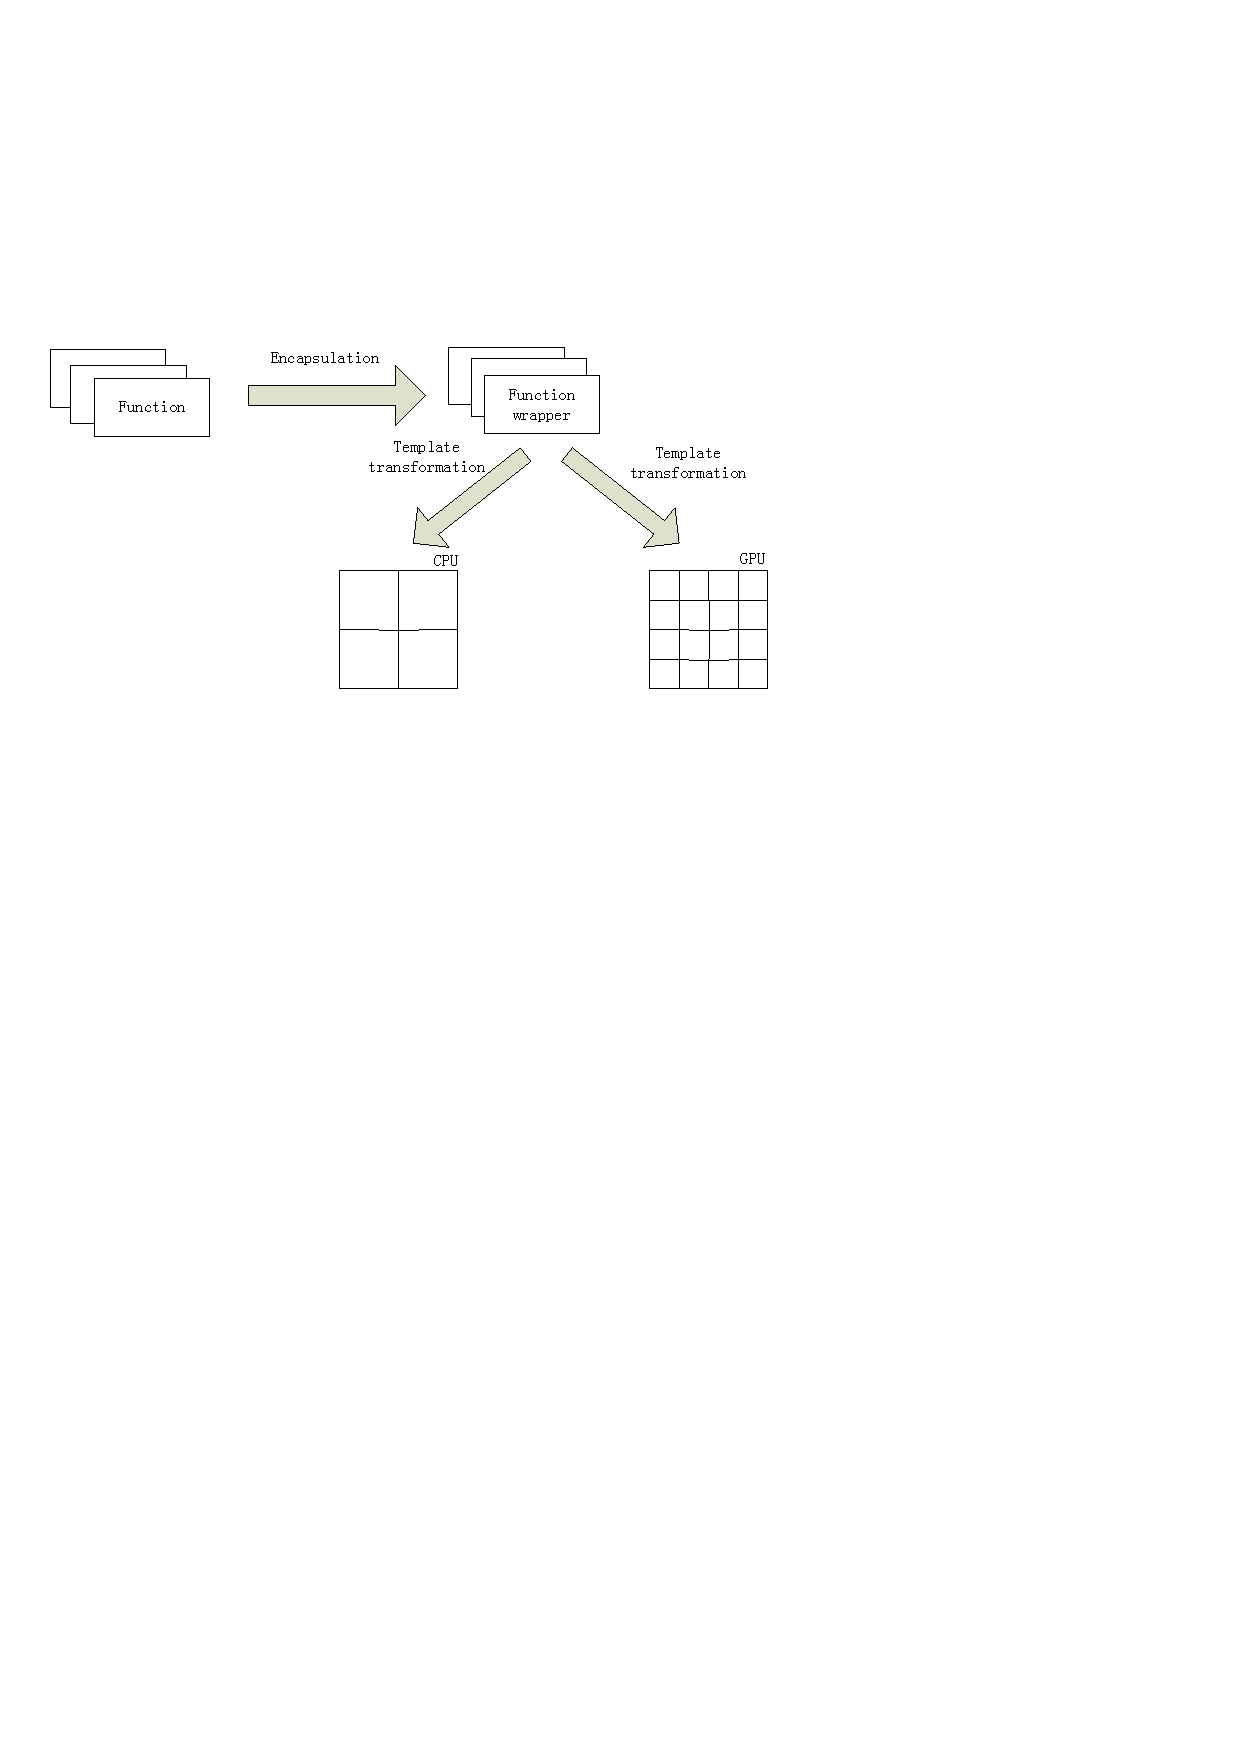
\includegraphics[width=3.3in]{../overview}
\caption{Overview of template-based programming model: Programmers
write side-effect free functions in C/C++, then encapsulate them in
template classes. Such a template encapsulate the computing function and can be 
automatically transformed into a
group of subtasks by TF classes based on appropriate parallel patterns. Finally,
subtasks directly run on physical multicores.}
\label{fig:overview}
\end{figure}

We propose a template metaprogramming approach to support parallel programms
running on different multi-core systems. \reffig{overview} gives an overview
of our approach: a side-effect free function is abstracted as a \emph{task}
and is wrapped in a template class. We provide template classes
to support different parallel patterns:

\begin{itemize}
\item \textbf{Hierarchy pattern.} A task is recursively divided into subtasks
and subtasks can execute on multiple cores in parallel.

\item \textbf{Pipeline pattern.} A task is divided into a series of processing
subtasks, where the output of a previous subtask is directly used as the input
of the next subtask and each subtask execute on a core.

\item \textbf{Map-Reduce pattern.} A task is divided into a map phase and a
reduce phase, where subtasks in each phase can execute in parallel on multiple
cores. The input of reduce phase is the output of the map phase.

\end{itemize}

The transformation from a task to parallel patterns is a
source-to-source conversion with C++ templates, which are called \emph{TF
class} in this paper (Section~\ref{sect:tf}).  The converted code calls
architecture-specific building block classes (Section~\ref{sect:bb}) so that
when compiled, a task can execute on
different multi-core systems in parallel at run time. 

The rest of this section first describes three class types of our approach, i.e.,
TF, view, and building block classes. 
%(1) View class, a representation of underlying containers such as vector or matrix.
%(2) Building block class,
%provide basic executions of tasks on multicores (3) TF class, each one
%represents a parallel pattern. 

\subsection{TF Classes}
\label{sect:tf}

A \textit{TF class} (short name for \textit{TransFormation class}) is a template
class representing a parallel pattern which transforms a task to a group of
subtasks in isomorphism. In other words, the transformed task has the same interface
while owns a call graph inside to complete the original computation by a
group of subtasks. Specifically, the following two classes are used in this paper: 

\begin{itemize} 
\item \textbf{TF\_hierarchy}. This template class recursively divides a task into subtasks
until certain predicate is evaluated as true. %As Fig.~\ref{fig:mmexample} depicted,  we use
In fact, \code{TF\_hierarchy} can implement a programming model similar to Sequoia and
we use \code{TF\_hierarchy} to implement both hierarchy and Map-Reduce pattern.

\item \textbf{TF\_pipeline}. This template class synthesizes a call chain of an
arbirary number of functions into a pipeline. This is a common pattern for
stream kernel programming model.
\end{itemize} 

\subsubsection{TF\_hierarchy}

\reffig{tf:code} illustrates the class definition of \code{TF\_hierarchy}. The
prime template (line 1 to 10) takes three parameters, i.e., user supplied \code{TASK}
class, a predicate class, and a bool value.
The predicate class is similar to Merge~\cite{merge} and is used to generate subtasks
recursively. The main difference from Merge is that our predicate is a
\emph{metafunction} and is evaluated in place: the bool value is evaluated at
compilation time and depends on the two types, \code{TASK::ARG0} and \code{TASK::ARG1},
defined in the class \code{TASK}. Usually these two types are views (Section~\ref{sec:view})
with statically known size. When the third parameter is evaluated as false, the
prime template is used and \code{doit} function invokes recursive
\code{TASK:inner} function, which divides a task into subtasks.
On the other hand, when the third parameter is evaluated as true, the partial
specialization template (line 12 to 19) is used, where \code{doit} function
invokes \code{TASK::leaf} function (leaf node, no recursion).


\begin{figure}[hbt]
  \inputsrc{tf.cc}
  \caption{Pseudo-code of class \code{TF\_hierarchy}.}
  \label{fig:tf:code}
\end{figure}

\begin{figure}[hpt]
  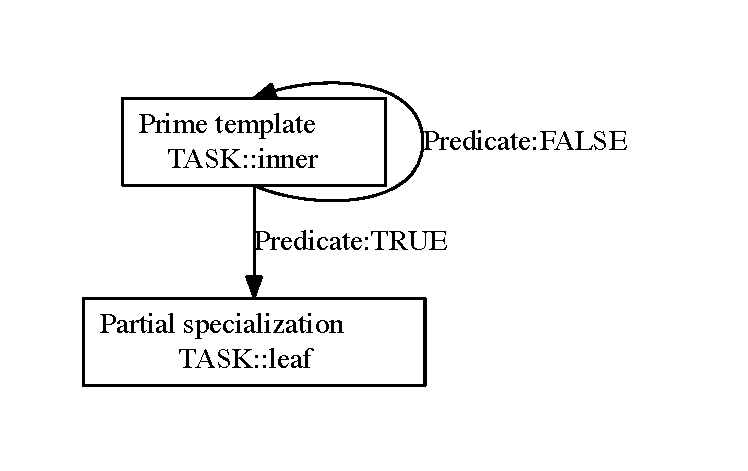
\includegraphics[width=3.0in]{../algo}
  \caption{Instantiation process of \code{TF\_hierarchy}. The predicate is a template
class, which is evaluted using \code{TASK}'s parameters.}
  \label{fig:hierarchy}
\end{figure}

The instantiation process of \code{TF\_hierarchy} is illustrated in \reffig{hierarchy}:
when predicate is false, the task is recursively divided into subtasks; when predicate
is true, the code (\code{TASK::leaf}) computes a subtask.

%A side-effect free function is referred to as \emph{task} in libvina. As a rule of thumb,
\todo{In this paper, we consider a class of computation-intensive functions (or tasks) that are 
self-contained, i.e., external data references are limited and
calling graphs of them are simple. For these functions, it's possible to
decouple a task into a cluster of subtasks. These subtasks are identical
except for arguments and we can distribute subtasks on multi-core to execute simultaneously. 
}

%We implement two TF classes in libvina though  it is not
%necessary to use TF classes to perform source transformations. We
%encourage to do so because it has engineering advantages, which reduces
%effects of system programmers.

\subsubsection{TF\_pipeline}
The \code{TF\_pipeline} class using variadic template~\cite{vartemp}, as
illustrated in \reffig{pipeline:code}. \code{TF\_pipeline} supports an arbitrary
number of functions chaining together and the only limitation is the maximal
level of template recursions of a compiler.

%For C++ compilers don't support variadic template, there
%are workarounds to achieve the same effect, but quite
%tedious.\footnote{zhangsq ask me to cite. I implemented the
 % workarounds myself, but i don't see it is necessary to show them here. too
 % details... --xliu 28. Nov}.

\begin{figure}[hbt]
  \inputsrc{pipeline.cc}
  \caption{Pseudo-code of class \code{TF\_pipeline}.}
  \label{fig:pipeline:code}
\end{figure}


\subsection{View Classes}
\label{sec:view}

A \emph{View} is a class representing a subset of container's data. For example,
a matrix type could have views that contains a subset of elements of a matrix.
There are two kinds of views, \code{ReadView} and \code{WriteView}.
A \code{ReadView} is read-only, while a \code{WriteView} allows write operations on its data
(by providing interfaces to write). 

To ensure multi-thread safety, \code{ReadViewMT} and \code{WriteViewMT} are
defined. For these two types, each object contains a signal that is copied across multiple
threads. All operations of \code{ReadViewMT} or \code{WriteViewMT} are blocked until the
current thread is signaled by other threads.

\reffig{view} depicts the relationship of views. Concrete lines means that
a type cast from a source node to a destination node is legal, i.e., an implicit
conversion in C++.  Dashed lines means a source node can generate objects of
the type of the destination node. Labels on the dashed line signifies how
signals are created or copied.
Shadow region is another thread space.

%The only approach to communicate with other
%threads is through a special kind of view called \emph{ViewMT}.  

The design of view class serves two purposes. 1) The classes are type-safe.
Because template instantiation is not visible for programmers, our
source transformations by templates may introduce subtle errors. We
expect compilers complain explicitly when unintentional
transformations happen. For example, when a \code{ReadView} is accidently used
for writes, the compiler will complain for errors. 2) View classes hide architecture specifics. %communication details. 
Implementations have choice to optimize data movement according to
architectures. Shared memory systems~\cite{larrabee} and communication-exposed
multicores~\cite{cellbe, imagine} usually have different strategies to perform
the operations. In fact, our implementation of for CPU and GPU are different (See
Section~\ref{sec:details}).

\begin{figure}
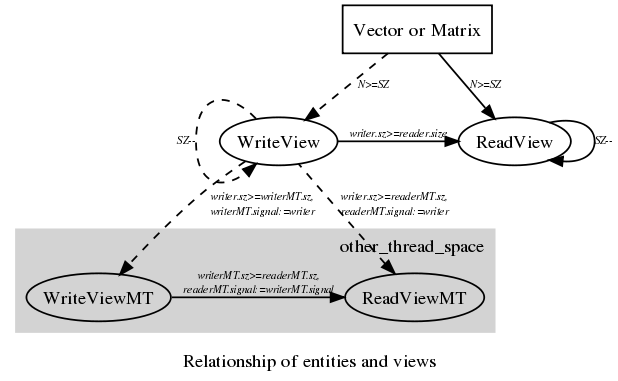
\includegraphics[width=3.6in, height=2.5in]{../relationship_views}
\caption{The relationship of view classes. A concrete line represents a valid
   type cast, while a dashed line represents a source node can generate objects
of the type pointed to. Labels specify how signals are created or copied
across views.}
\label{fig:view}
\end{figure}


\subsection{Building Block Classes}
\label{sect:bb}

\begin{table}[hbt]
\caption{Building block classes in libvina}
\begin{tabular}{|c|l|l|}
\hline
Name& Semantics& Usage Example\\
\hline
\textbf{par$<$T, K, F$>$}& Iterate function \textit{F} \textit{K} times &par$<$\_tail, 4, F$>$\\ 
                         &in parallel, implicit barrier                 &::apply();\\                
\hline
\textbf{seq$<$T, K, F$>$}& Iterate function \textit{F} \textit{K} times&seq$<$\_tail, 5, F$>$\\
                         &                                             &::apply();\\
\hline
\textbf{reduce$<$K, F$>$}&Reduce \textit{K} values using &reduce$<$8, F$>$\\
&function
\textit{F}&::apply(values)\\
\hline
\textbf{mt::thread$<$F$>$}&Spawn a thread to execute  & mt::thread$<$F$>$\\
                          &function \textit{F}        & ::apply();\\
%\textbf{do\_}&loop until predicate is evaluated true.& 
\hline
\end{tabular}\label{tbl:bb}
\end{table}

A building block class is a high-level abstraction of execution patterns that
hide architecture-specific details. Programmers can use building blocks to
execute tasks on different multi-core platforms.
\reftable{bb} lists building blocks in libvina. For tasks that can
executed in SPMD (Single-Program-Multiple-Data) fasion, \code{par} class spawns
multiple threads to execute subtasks in parallel. \code{seq} class supports
pipeline patterns. Parameter $T$ in \code{par} or \code{seq} could be nested
\code{par}, nested \code{seq}, or \code{\_tail} (meaning no further nestings).
For instance, we can write the following statement 

%However, if it is
%not the case, we have to deal with dependences carefully using \code{seq} and \code{reduce}. 
%Like traditional programming languages, our
%building blocks of iterations support nesting definition. In addition, both \textit{seq} and
%\textit{par} are interoperable. 

\begin{lstlisting}
seq<par<_tail, 4>, 3, F>::apply();
\end{lstlisting}
to build to a two-level loop, and the nested loop are executed in
parallel. The equivalent OpenMP code is:
\begin{lstlisting}
F f;
int i, j;
for (i=0; i<3; ++i)
{
  #pragma omp parallel private(j)
  for (j=0; j<4; ++j) 
    f(i, j);
}//implicit barrier
\end{lstlisting}

%The first template parameter $T$ of iterations is used to support nest. It could be
%either a par or a seq. Special classes \code{par\_tail} and \code{seq\_tail} are
%symbols to indicate the end of nest.

The \code{reduce} class supports the ``reduce'' pattern in MapReduce style tasks.
Specifically, a given function $F$ is used to reduce $K$ input values and the
final result is stored in the first value. Note that many of the $K-1$ times
reduce operations are executed in parallel using multiple threads.

Finally, \code{mt::thread} class provides a thread interface for programmers to
dynamically spawn a new thread to execute a function.

%can exploit it to bind thread directly (\textit{e.g.} line 19 of List 2)
%or develop other customized building blocks.



%programming model
\comment{
We use template metaprogramming to implement a parallel programming model.
Essentially, our approach utilizes C++ template mechanism to
perform source-to-source transformations for multicores. Side-effect
free functions are abstracted as \emph{tasks}. A task is
wrapped in the form of template class, named \emph{function
  wrapper}.  A \emph{TF class} is a template class, which
is capable of transforming a task into a group of subtasks based on
a parallel pattern. Tasks
apply TF classes according to their appropriate
parallel patterns. This process is called ast \emph{adaption}. 
Finally, we use \emph{building block classes} to define executions of tasks
on specific architectures. Both TF classes and building
blocks are organized as a library --
\textbf{libvina}.}


